\section{Geometries, tensor exchange and conformance mutants}\label{sec:supp-moved}

\subsection{The three geometries}
Figure~\ref{fig:structures} of the main text draws the survey slab, CuH\(_2\) and the EMT hop.

\subsection{The hop drawings}
Figure~\ref{fig:claisen-struct-ids} of the main text is the \(4\times 4\) top view.
The hydrogen is blue, the CON rows of two copper atoms are red, and the inset is the side view.

\subsection{Zero-copy tensor exchange}
A caller that already has a frame should read its coordinates as a tensor.
readcon-core exposes that tensor through DLPack \cite{dlpackDLPack2026}.
On the Rust builder the methods for positions, velocities, forces, per-atom energies and masses return a borrowed float64 tensor, and the method for atom identifiers returns a borrowed uint64 tensor.
The lifetime of each borrowed tensor is the builder, and the default build places it on the CPU.
A C caller that needs the tensor after the builder is gone takes the versioned managed tensor, and that export copies the storage.
Python materialises a contiguous NumPy array, and that array implements the DLPack protocol, so PyTorch, JAX and CuPy take the array with no second copy.
The measured exchange is a NumPy DLPack view against an explicit copy of the same positions, for \dlpackAtoms{} copper atoms.
Each arm is eight repeats.
The view takes a median of \SI{4.0}{\micro\second} and the copy a median of \SI{32}{\micro\second}, so the view costs 0.12 times the copy.
A 95 percent interval for that ratio is 0.11 to 0.15.
The type 7 interquartile ranges are \SI{0.77}{\micro\second} and \SI{1.2}{\micro\second}.
Figure~\ref{fig:dlpack} shows the eight repeats.

\begin{figure}[tbp] \centering
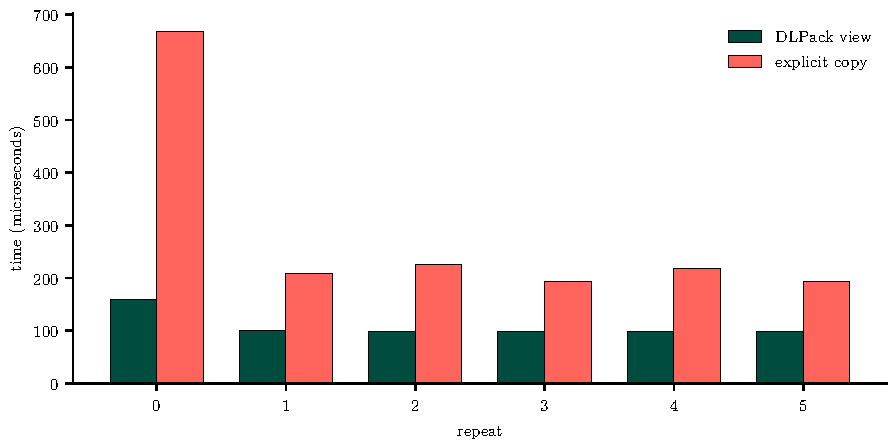
\includegraphics[width=\textwidth]{figures/generated/dlpack.pdf}
\caption{Eight repeats of a DLPack view and an explicit copy of 32768 positions.
The view median is 4.0 microseconds and the copy median is 32 microseconds.}
\label{fig:dlpack} \end{figure}

\subsection{Mutants and the extended XYZ drift}
The two readers read \(\mutantCases\) mutants of the \(\mutantFiles\) corpus files under \(\mutantMaxBytes\) bytes, \(\mutantPerSeed\) from each of \(\mutantSeeds\) seeds, each made by inserting, deleting or replacing characters and tokens at one to three random places.
They agree on \(\mutantSame\) of them, with the same frame count or error class.
The count-line rule accounts for all 15 differences.

The release runs 140 differential cases mutated from its test files and its conformance corpus.
Every case is read from a string, from bytes, from a plain and a gzip file at one to sixteen threads, through the column readers and through the stream reader, and each read returns the frame count, coordinates and section presence of the one-thread string read or stops with its error at the same line.

The outcomes of the published wheels of readcon-core \driftWheels{} on the probe files are in Section~\ref{sec:supp-versions}.
Table~\ref{tab:versions} lists the clauses those readings concern.

Extended XYZ is the text format set beside CON, because it publishes a grammar.
Table~\ref{tab:drift} gives seven three-atom files to \(\driftAllPaths\) reader paths from \(\driftAllLibraries\) libraries.
On the reference frame the \(\driftXyzPaths\) extended XYZ paths, from \(\driftXyzLibraries\) libraries, return \(\driftXyzOutcomes\) different outcomes.
That grammar admits a \texttt{d} or \texttt{D} exponent and reads \texttt{T}, \texttt{true}, \texttt{True} and \texttt{TRUE} as true, and the paths split on both files.
It leaves open whether a comment line that is not key-value pairs makes a file plain XYZ or an error, and on such a file the default C path of libAtoms departs from the default periodicity while its Python parser fails.
From extxyz 0.4.2 the C reader defaults to a whitespace split, with \texttt{use\_regex} false, and extxyz 0.4.6 keeps that default on \texttt{read\_dicts} \cite{kermodeExtxyz0422026}.
The package ase-extxyz 0.1.2 registers that C parser with ASE as the format \texttt{cextxyz} \cite{kermodeAseExtxyz0122026}.
The ASE extended XYZ arm in the 0.22.0 measurements calls \texttt{format='extxyz'}, the reader shipped in ASE 3.29.0, not \texttt{cextxyz}.
extxyz-ng 0.0.2 is a Rust reader with Python bindings \cite{yuExtxyzNg0022026}.
Section~\ref{sec:h2h} times these readers, and the writers that provide a write call, on one set of files.

\subsection{The Morse band}
\begin{figure}[tbp] \centering
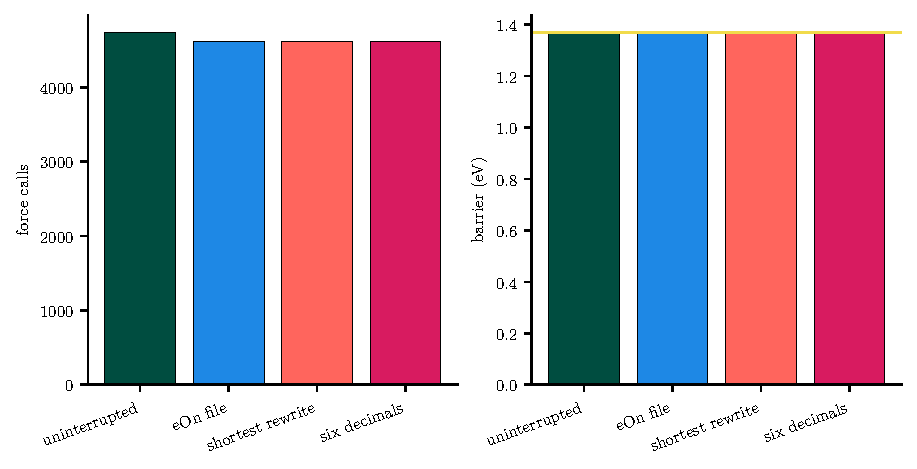
\includegraphics[width=\textwidth]{figures/generated/restart.pdf}
\caption{Morse band. Energy of each image above the first. The uninterrupted band and the round trip overlie each other, and six decimals lies on the same profile. The barrier is 1.37~eV.}
\label{fig:restart} \end{figure}

\section{readcon-db keys and commands}\label{sec:supp-tools}
A frame key is 12 bytes: the trajectory id as a big-endian 64-bit integer, then the frame index as a big-endian 32-bit integer.
The record is the CON text, optionally compressed with zstd \cite{colletZstandardCompressionApplicationzstd2021}.
The exact identity of a frame is the xxHash3-128 of that text.
\texttt{index-canonical} reorders the frame into increasing \texttt{atom\_id}, under the strict check of symbol, mass and fixed mask, and stores the xxHash3-128 of that round-trip text.
\texttt{find-by-atom-order} returns each stored frame with that hash and the permutation from the query, so a band image grouped by element is the same saddle.
The indexes are the atom count, the symbol, the element counts, the formula, as in \texttt{Cu:2|H:2}, the energy, the maximum force, the mass, the volume, the periodic flags, the metadata, the flags and the topology.
The metadata holds the time, the NEB bead and the band, the charge and the magnetic moment.
\texttt{annotate-topology} runs the d-SEAMS fingerprint, a cutoff graph to two hops, with nauty or a Weisfeiler--Lehman colouring.
The resulting key names the bonded graph up to relabelling: a rooted-neighbourhood certificate on each atom, and a ring census \cite{trochetDiffusionPointDefects2015}.
That key is separate from the byte hash.
\texttt{select} takes \texttt{-{}-formula}, \texttt{-{}-require-*}, \texttt{-{}-topo-key} and \texttt{-{}-neb-bead-*}.
The corpus is also a Python module and a C and Fortran interface.

\section{Cell angles and decimal paths}\label{sec:supp-cell}
In binary64 the cosine of the double nearest \(\pi/2\) is \(\num{\wkCosRight}\), so Eq.~\eqref{eq:cell} gives this cell \(b_x=\num{\wkBx}\,\text{\AA}\) and \(c_x=c_y=\num{\wkCxy}\,\text{\AA}\).
ASE~\wkAseVersion{} returns \(b_x=\wkAseRightBx\), because it sets the cosine of an angle within two units in the last place of a right angle to zero \cite{larsenAtomicSimulationEnvironmenta2017}.
The exact \(\rho\) is zero for angles of \(\wkFlatAlpha\), \(\wkFlatBeta\) and \(\wkFlatGamma\) degrees, since \(\mathbf{c}\) then lies in the plane of \(\mathbf{a}\) and \(\mathbf{b}\), and binary64 gives \(\hat\rho=\num{\wkFlatRadicand}\).
readcon-core accepts that frame with \(c_z=0\), because \(\hat\rho\) lies inside the window of \(\num{\wkWindow}\) that Section~\ref{sec:format} gives for the roundoff of a zero radicand, and ASE stops on its own assertion that \(\hat\rho\ge0\).
With \(\wkNoneAlpha\), \(\wkNoneAlpha\) and \(\wkNoneGamma\) degrees, \(D=\wkNoneGram\) and \(\rho=\wkNoneRadicand\).
readcon-core rejects that frame with an error that names line~\trCellLine, and ASE fails the same assertion without naming a line.

The shortest decimal uses \wkDigitsMin{} to \wkDigitsMax{} significant digits, and the reader rounds each decimal to the nearest binary64 value \cite{lemireNumberParsingGigabytes2021}.
A writer that prints six decimals instead puts \(x=\wkFirstXRounded\) in line~\wkLineFirstRow, a shift of \(\num{\wkShiftFirst}\,\text{\AA}\), and moves the \wkCoordinates{} coordinates by up to \(\num{\wkShiftMax}\,\text{\AA}\).
Resumed from six decimals, the climbing-image band of Section~\ref{sec:cases} converges in the same step count with its barrier moved by \(\num{\rfDeSixNum}\,\mathrm{eV}\).

The first four bytes select the envelope.
A gzip stream is inflated into memory, and a zstd stream is inflated when the build includes that decoder.
A plain file shorter than \SI{64}{\kibi\byte} is read into memory.
A longer plain file stays mapped for the position-block reader.
The read of the whole file loads the bytes into one buffer on every size.
With one worker, the boundary thread then parses the frames in order.
With two or more workers, and a build that includes the pool, each worker parses its own span and the frames come back in file order.

\begin{figure*}[tbp]
\centering
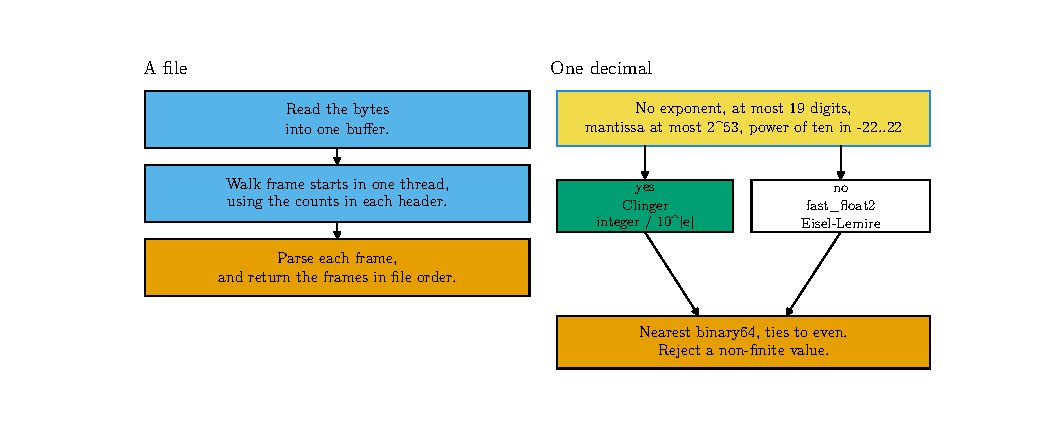
\includegraphics[width=\textwidth]{figures/generated/parser.pdf}
\caption{Left: one thread finds the frame starts from the counts, then the frames are parsed in file order.
Right: a short decimal takes Clinger's conversion, and every other spelling takes \texttt{fast\_float2}.
Both paths round to the nearest binary64 value.}
\label{fig:parser}
\end{figure*}

A coordinate row is three decimals, a mask and an optional identifier, scanned once.
Clinger's conversion applies when the spelling has no exponent marker, at most 19 digits, a mantissa of at most \(2^{53}\), and a power of ten from \(-22\) to \(22\) \cite{clingerHowReadFloating1990}.
The mantissa is an integer that binary64 represents exactly.
Division or multiplication by the matching power of ten, taken from the same table \texttt{fast\_float2} uses, produces the value.
A sign is applied after the scaling.
Any other spelling, including a decimal with \texttt{e} or \texttt{E}, is parsed by \texttt{fast\_float2}, an Eisel--Lemire conversion \cite{lemireNumberParsingGigabytes2021}.
A non-finite result is rejected on both paths.
The two paths agree bit for bit on the spellings the short path accepts.
The mask is then an integer, 0 or 1 in version 1 and 0 through 7 from version 2, and the identifier is a decimal integer that does not pass through binary64.
Section~\ref{sec:fast} compares the two builds.

\section{Cross-library round trips}\label{sec:supp-rounds}
The reads in Section~\ref{sec:host} use the library built for that host.
We first wrote the survey frame of Listing~\ref{lst:frame} with one library and read it back with the same library or another, \(\surveyRoutes\) routes in all, \(\surveySameRows\) within one library and \(\surveyCrossRows\) across two (Table~\ref{tab:survey}).
The libraries are ASE \cite{larsenAtomicSimulationEnvironmenta2017}, chemfiles \cite{frauxChemfileschemfilesVersion01042023}, MDAnalysis \cite{gowersMdanalysisPythonPackage2016,gowersMdanalysis21102026}, h5py, OVITO \cite{stukowskiVisualizationAnalysisAtomistic2010} and Open Babel \cite{oboyleOpenBabelOpen2011}, at the versions of Section~\ref{sec:supp-versions}, and each stores each field through the mechanism its documentation gives.
We grade a returned field as fixed by the format when the format's own specification defines its place in the file, and as a convention when only the documented layout of a library defines that place.
The ASE trajectory, with the identifiers stored as ASE tags, and H5MD written and read with h5py also return every field bit for bit.
The trajectory keeps the mask, the identifiers, the unit and the periodicity in the layout of ASE, and H5MD keeps the mask in a dataset outside the H5MD specification, which only our reader knows to read.
Extended XYZ returns the mask and the identifiers through the column names of ASE, which chemfiles and OVITO also read.
ASE writes that file with eight decimals, a shift of \(\num{\surveyAseXyzShiftNum}\,\text{\AA}\); chemfiles 0.10.4 moves the coordinates by \(\num{\surveyChemXyzShiftNum}\,\text{\AA}\), rounds the cell lengths to six significant digits and drops the velocities.
chemfiles 0.10.4 stores one cell vector per column of the cell matrix.
MDAnalysis 2.11.0 returns single precision on the H5MD file, which changes a coordinate by up to \(\num{\surveyMdaShiftNum}\,\text{\AA}\), and Open Babel keeps the identifiers only inside the site labels of a Crystallographic Information File (CIF).
That float32 shift stays with the H5MD reader of release 2.11.0.
Release 2.11.0, of 2026-10-21, reads one PDBx/mmCIF frame through gemmi and converts the positions and velocities of a GROMACS TPR file into its base units \cite{gowersMdanalysis21102026}.
Identifiers come back on \(\surveyCrossIds\) of the \(\surveyCrossRoutes\) cross-library round trips, all through the \texttt{id} column of ASE.

\section{The velocity unit of a misread}\label{sec:supp-velunit}
A \(\velFixtureAtoms\)-atom fixture stores velocities in the declared natural unit.
Its kinetic energy is \(\velFixtureKe\,\mathrm{eV}\) in that unit and \(\velFixtureKeFs\,\mathrm{eV}\) with the same numbers read as \(\text{\AA}/\mathrm{fs}\), the factor \(\velFactorSq\) of Eq.~\eqref{eq:tau}.
After one velocity Verlet step of 1~fs \cite{swopeComputerSimulationMethod1982}, the misread positions differ from the declared ones by \(\velVerletRmsd\,\text{\AA}\) root mean square and by at most \(\velVerletMax\,\text{\AA}\) (Section~\ref{sec:supp-velocity}).
A \(\velSlabAtoms\)-atom slab drawn at \(\velSlabTemperature\,\mathrm{K}\) has a kinetic energy of \(\velSlabKe\,\mathrm{eV}\), and the misread gives \(\num{\velSlabKeFsNum}\,\mathrm{eV}\).

\section{The mW nucleation window}\label{sec:supp-water}
The trajectory is an ice Ih slab of \mwMolecules\ mW molecules, with a 10~fs step.
It is relaxed for \mwRelaxPs~ps in the NPT ensemble at \mwRelaxK~K and zero pressure.
The upper \mwMeltFrac\ of the slab is melted for \mwMeltPs~ps at \mwMeltK~K while the rest is held fixed, and the system then runs in the NVT ensemble at \mwHoldK~K with a 200~fs damping time, in \mwLammps.
The analysed window is 81 frames, one per picosecond, from that NVT segment.
The neighbour cutoff is \(3.5\,\text{\AA}\), and the ice label is the CHILL+ class from the \(q_3\) bond correlation.
The CON frames store the orthorhombic cell, three dump-box lengths and right angles, and the XYZ comment line repeats that cell.
Figure~\ref{fig:water} is rebuilt from the four lags by
{\small\begin{verbatim}
python3 -c "import make_figures as m; m.water_persistence()"
\end{verbatim}}
